\section{SIB-Programmierung}

\subsection*{}
\begin{frame}{SIB-Programmierung}
	\begin{center}
		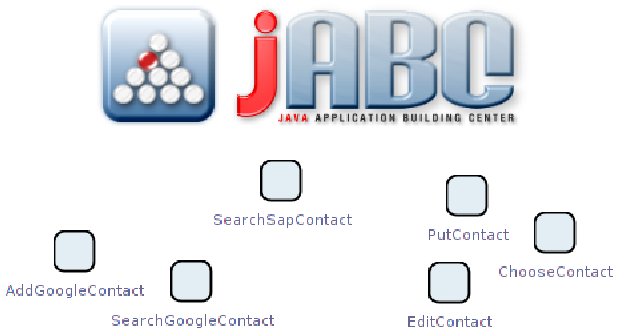
\includegraphics[width=\textheight]{Bilder/titel_sibs.png} 
	\end{center}
\end{frame}


\begin{frame}{Vorüberlegungen}
\begin{itemize}[<+->]
	\item \textbf{3 Sorten von SIBs:} Google, SAP, GUI
	\pause
	\item \textbf{Google-SIBs:} Kontakt suchen und hinzufügen
	\item \textbf{SAP-SIB:} Kontakt suchen
	\pause	
	\item \textbf{GUI-SIBs:} 
		\begin{itemize}[<+->]
			\item Eingabe von Kontakt-Attributen
			\item Auswahl aus einer Liste von Kontakten
		\end{itemize}
	
\end{itemize}
\end{frame}



\subsection*{SIBs im Detail}
\begin{frame}{Google + SAP: suche Kontakt}
\begin{itemize}[<+->]
	\item \textbf{Input:} eine Instanz der Klasse \texttt{Contact} 
		\begin{itemize}[<+->]
			\item dient als Filter für die Suche
		\end{itemize}
	\item \textbf{Output:} Liste von \texttt{Contact}-Objekten

	\item \textbf{Branches:} 
		\begin{itemize}[<+->]
			\item \textbf{found:} mehr als 0 Ergebnisse
			\item \textbf{not found:} keine Ergebnisse
			\item \textbf{error:} es wurde eine \textit{Exception} geworfen
		\end{itemize}
	
\end{itemize}
\end{frame}


\subsection*{SIBs im Detail}
\begin{frame}{Google: Kontakt hinzufügen}
\begin{itemize}[<+->]
	\item \textbf{Input:} eine Instanz der Klasse \texttt{Contact} 

	\item \textbf{Output:} keiner

	\item \textbf{Branches:} 
		\begin{itemize}[<+->]
			\item \textbf{default:} Kontakt erfolgreich hinzugefügt
			\item \textbf{error:} es wurde eine \textit{Exception} geworfen
		\end{itemize}
	
\end{itemize}
\end{frame}


\subsection*{SIBs im Detail}
\begin{frame}{GUI: Kontakt-Daten eingeben}
\begin{itemize}[<+->]
	\item \textbf{Input:} eine Instanz der Klasse \texttt{Contact} 
		\begin{itemize}[<+->]
			\item Formular wird entsprechend befüllt
			\item zudem Parameter für Fenstertitel und Validierung
		\end{itemize}
	\pause
	\item \textbf{Output:} geänderte(!) Instanz der Klasse \texttt{Contact}
		\begin{itemize}[<+->]
			\item wenn Button "OK" geklickt wurde
		\end{itemize}
	\pause	
	\item \textbf{Branches:} 
		\begin{itemize}[<+->]
			\item \textbf{ok:} Eingabe bestätigt mit Button "OK"
			\item \textbf{cancel:} Eingabe abgebrochen mit Button "CANCEL"
			\item \textbf{error:} es wurde eine \textit{Exception} geworfen, oder UNKNOWN
		\end{itemize}
	
\end{itemize}
\end{frame}


\subsection*{SIBs im Detail}
\begin{frame}{GUI: Kontakt-auswählen}
\begin{itemize}[<+->]
	\item \textbf{Input:} Liste von \texttt{Contact}-Objekten 
		\begin{itemize}[<+->]
			\item zudem Parameter für Fenstertitel
		\end{itemize}
	\item \textbf{Output:} eine Instanz der Klasse \texttt{Contact}
		\begin{itemize}[<+->]
			\item wenn Button "OK" geklickt wurde
		\end{itemize}
	
	\item \textbf{Branches:} 
		\begin{itemize}[<+->]
			\item \textbf{ok:} Eingabe bestätigt mit Button "OK"
			\item \textbf{cancel:} Eingabe abgebrochen mit Button "CANCEL"
			\item \textbf{error:} es wurde eine \textit{Exception} geworfen, oder UNKNOWN
		\end{itemize}
	
\end{itemize}
\end{frame}


\subsection*{Probleme im Detail}
\begin{frame}[fragile]{Besonderheit der GUI}
\begin{itemize}[<+->]
	\item \textbf{warten auf Eingabe:} wie \texttt{trace()}-Methode anhalten? 
		\begin{itemize}[<+->]
			\item Swing-Frame läuft in einem eigenem Thread!
		\end{itemize}
	\pause		
	\item \textbf{Lösung hier:} mittels \texttt{synchronized})-Block in Frame und SIB
\end{itemize}
		
	\begin{lstlisting}
	public String trace(ExecutionEnvironment env) {

		...
		synchronized (frame) {
			frame.wait();
			...
	\end{lstlisting}
	
\begin{itemize}[<+->]	
	\item \textbf{Vorgehen:} 
		\begin{itemize}[<+->]
			\item \texttt{trace()} erstellt den Frame und wartet auf ein \texttt{notify()}
			\item \texttt{notify()} wird vom Action-Listener der Buttons aufgerufen
			\item im Anschluss kann \texttt{trace()} die Eingabe vom Frame erfragen
		\end{itemize}
\end{itemize}
\end{frame}


\subsection*{Probleme im Detail}
\begin{frame}{Problem mit jABC}
\begin{itemize}[<+->]
	\item \textbf{eigener Java-Code im jABC:} Unterschiede zum "normalen" JRE 
	\begin{itemize}[<+->]
			\item Code läuft ausserhalb von jABC...
			\item ABER: Ausführung im Modell wirft Exceptions?
	\end{itemize}
	\pause	
	\item \textbf{Lösung hier:} mittels "bad Practice"
\end{itemize}		
	\begin{lstlisting}
		...
		System.setProperty("javax.xml.parsers.SAXParserFactory", ...);
        System.setProperty("javax.xml.parsers.SAXParser", ...);
        System.setProperty("oracle.xml.parser.v2.SAXParser", ...);
        ...
	\end{lstlisting}
\begin{itemize}[<+->]	
	\item \textbf{Effekt:} 
		\begin{itemize}[<+->]
			\item verstellt Optionen der aktiven JVM
			\item auch nach Ausführung des Modells weiterhin wirksam
			\item sollte in realem Szenario vermieden werden
		\end{itemize}
\end{itemize}
\end{frame}


\section{jABC-Modell}

\subsection*{}
\begin{frame}{Modell und Anwendung}
\begin{center}
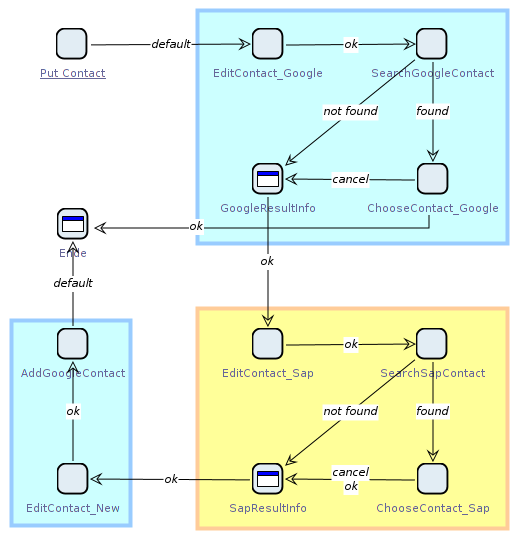
\includegraphics[width=\textheight]{Bilder/jabc_Model.png} 
\end{center}
\end{frame}



